\chapter{Экспериментальное исследование и обработка результатов}\label{chapter41}

\section{Постановка эксперимента}

\subsection{Конфигурация экспериментального стенда}

\subsubsection{Аппаратное обеспечение}

Процессоры 2 x Intel Xeon Platinum 8168 CPU @ 2.7 GHz.
Технология Hyper-Threading отключена для уменьшения нежелательного влияния на время обслуживания заявок в системе \cite{LowLatencyHT}.

Оперативная память: DDR4-2666 128 GiB.

\subsubsection{Программное обеспечение}

Операционная система Red Hat Enterprise Linux Server release 7.8 (Maipo).
Ядро Linux 3.10.0-1127.el7.x86\_64

Компилятор C++ Clang 6.0.1.

Стандартная библиотека C++: libstdc++ 8.1.0.

Библиотека Boost.Interprocess 1.68.0.

\subsection{Конфигурация экспериментальной системы}

Система для проведения эксперимента состоит из двух процессов:
\begin{itemize}
\item Процесс-шлюз отвечает за преобразование заявок из формата внешнего мира во внутренний формат системы и обратно. 
\item Процесс-обработчик совершает некоторые преобразования над заявкой и отправляет результат за пределы системы через процесс-шлюз.
\end{itemize}

Процессы выполняются на двух процессорах, расположенных в разных разъемах на материнской плате физического узла.

Снаружи системы находится симулятор внешнего мира. Он генерирует поток заявок в систему и получает результат обработки заявки в системе. Схема взаимодействия процессов в эксперименте представлена на рисунке \ref{chapter41:SystemSchema}.

\begin{figure}[!h]
\caption{Схема взаимодействия процессов в эксперименте}
\label{chapter41:SystemSchema}
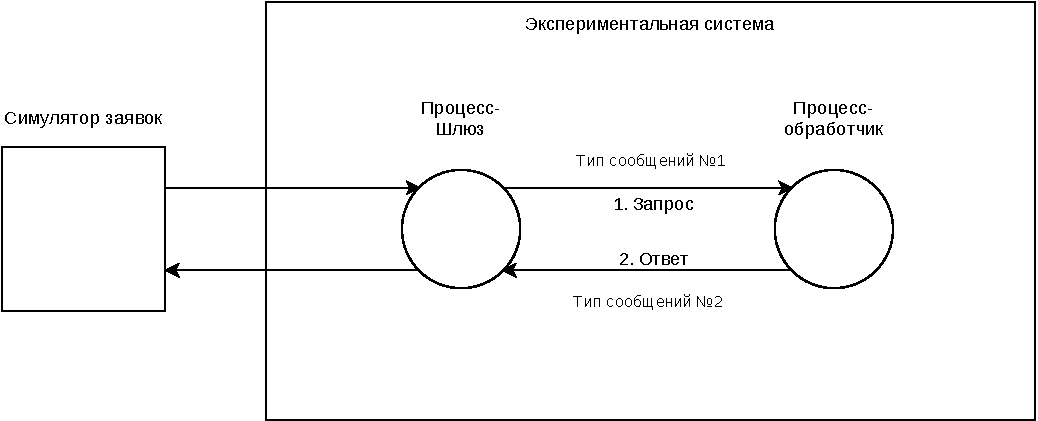
\includegraphics[width=\textwidth]{../../graphics/schemes/SystemSchema}
\end{figure}

В настоящей работе замеряется временная задержка на передачу данных между процессами внутри системы, а именно из процесса-шлюза в процесс-обработчик и обратно (сообщения типа №1 и №2 в запросе и ответе между процессом-шлюзом и процессом обработчиком на рисунке \ref{chapter41:SystemSchema}).

Процессы системы взаимодействуют используют одно соединение, в рамках которого заявки обрабатываются строго последовательно.
Обслуживание включает в себя: прием заявки, выполнение пользовательской логики над заявкой и, если необходимо, отправка ответа.
Временной задержкой на передачу данных в настоящей работе принимается временной промежуток от начала отправки заявки до \textbf{начала обработки заявки}. Таким образом, возможен случай, когда во время обработки очередной заявки процессом в очереди уже находится следующая заявка, временная задержка на передачу которой, таким образом, увеличится на время обработки текущей заявки.

Данный сценарий актуален для процесса-обработчика, в котором обслуживание заявки осуществляется непосредственно в транспортном потоке
В случае с процессом-шлюзом транспортный поток только читает и диспетчеризует асинхронную обработку заявки, т.е. не выполняет обработку самой заявки.

\textbf{TBD: надо как- то адекватно это описать}
Пользовательская логика процесс-обработчика в среднем отклоняет 25\% заявок, в то время как 75\% заявок отправляются в процесс-шлюз.

\subsection{Используемые обозначения}

\begin{itemize}
\item $\Delta$ -- временная задержка между сериями заявок;
\item $\delta$ -- временная задержка между заявками в серии;
\item $\tau$ -- временная задержка на передачу данных;
\item $T$ -- время обслуживания заявки.
\item транспортный поток -- поток из пула транспортных потоков, непосредственно обслуживающий получаемые заявки.
\end{itemize}

Из-за сложного характера распределений для представления полученных данных используются гистограммы выборок и 50, 80, 90, 95 и 99 процентили.

\subsection{Характер экспериментальной нагрузки}

Характеристики потока заявок, создаваемого симулятором, приведены в таблице \ref{chapter41:TableSimulator}.
\begin{table}[!h]
\caption{Процентили интервалов между сериями заявок и заявками, создаваемыми симулятором}\label{chapter41:TableSimulator}
\centering
\begin{tabular}{|l|l|l|l|l|l|l|l|}
\hline
Процентиль & 0\% & 50\% & 80\% & 90\% & 95\% & 99\% & 100\% \\ \hline
$\Delta$, мс & 5 & 9 & 11 & 12.5 & 13 & 15 & 109 \\ \hline
$\delta$, мкс & 52 & 62 & 82 & 110 & 115 & 128 & 4819 \\ \hline
\end{tabular}
\end{table}

\subsection{Время обслуживания заявок в процессах}

На рисунке \ref{chapter41:EngineLatency} представлена гистограмма времени обслуживания заявок в процессе-обработчике. В таблице \ref{chapter41:TableEngine} представлены процентили времени обслуживания заявок в процессе-обработчике.
\begin{figure}[!h]
\caption{Гистограмма времени обслуживания заявки в процессе-обработчике}
\label{chapter41:EngineLatency}
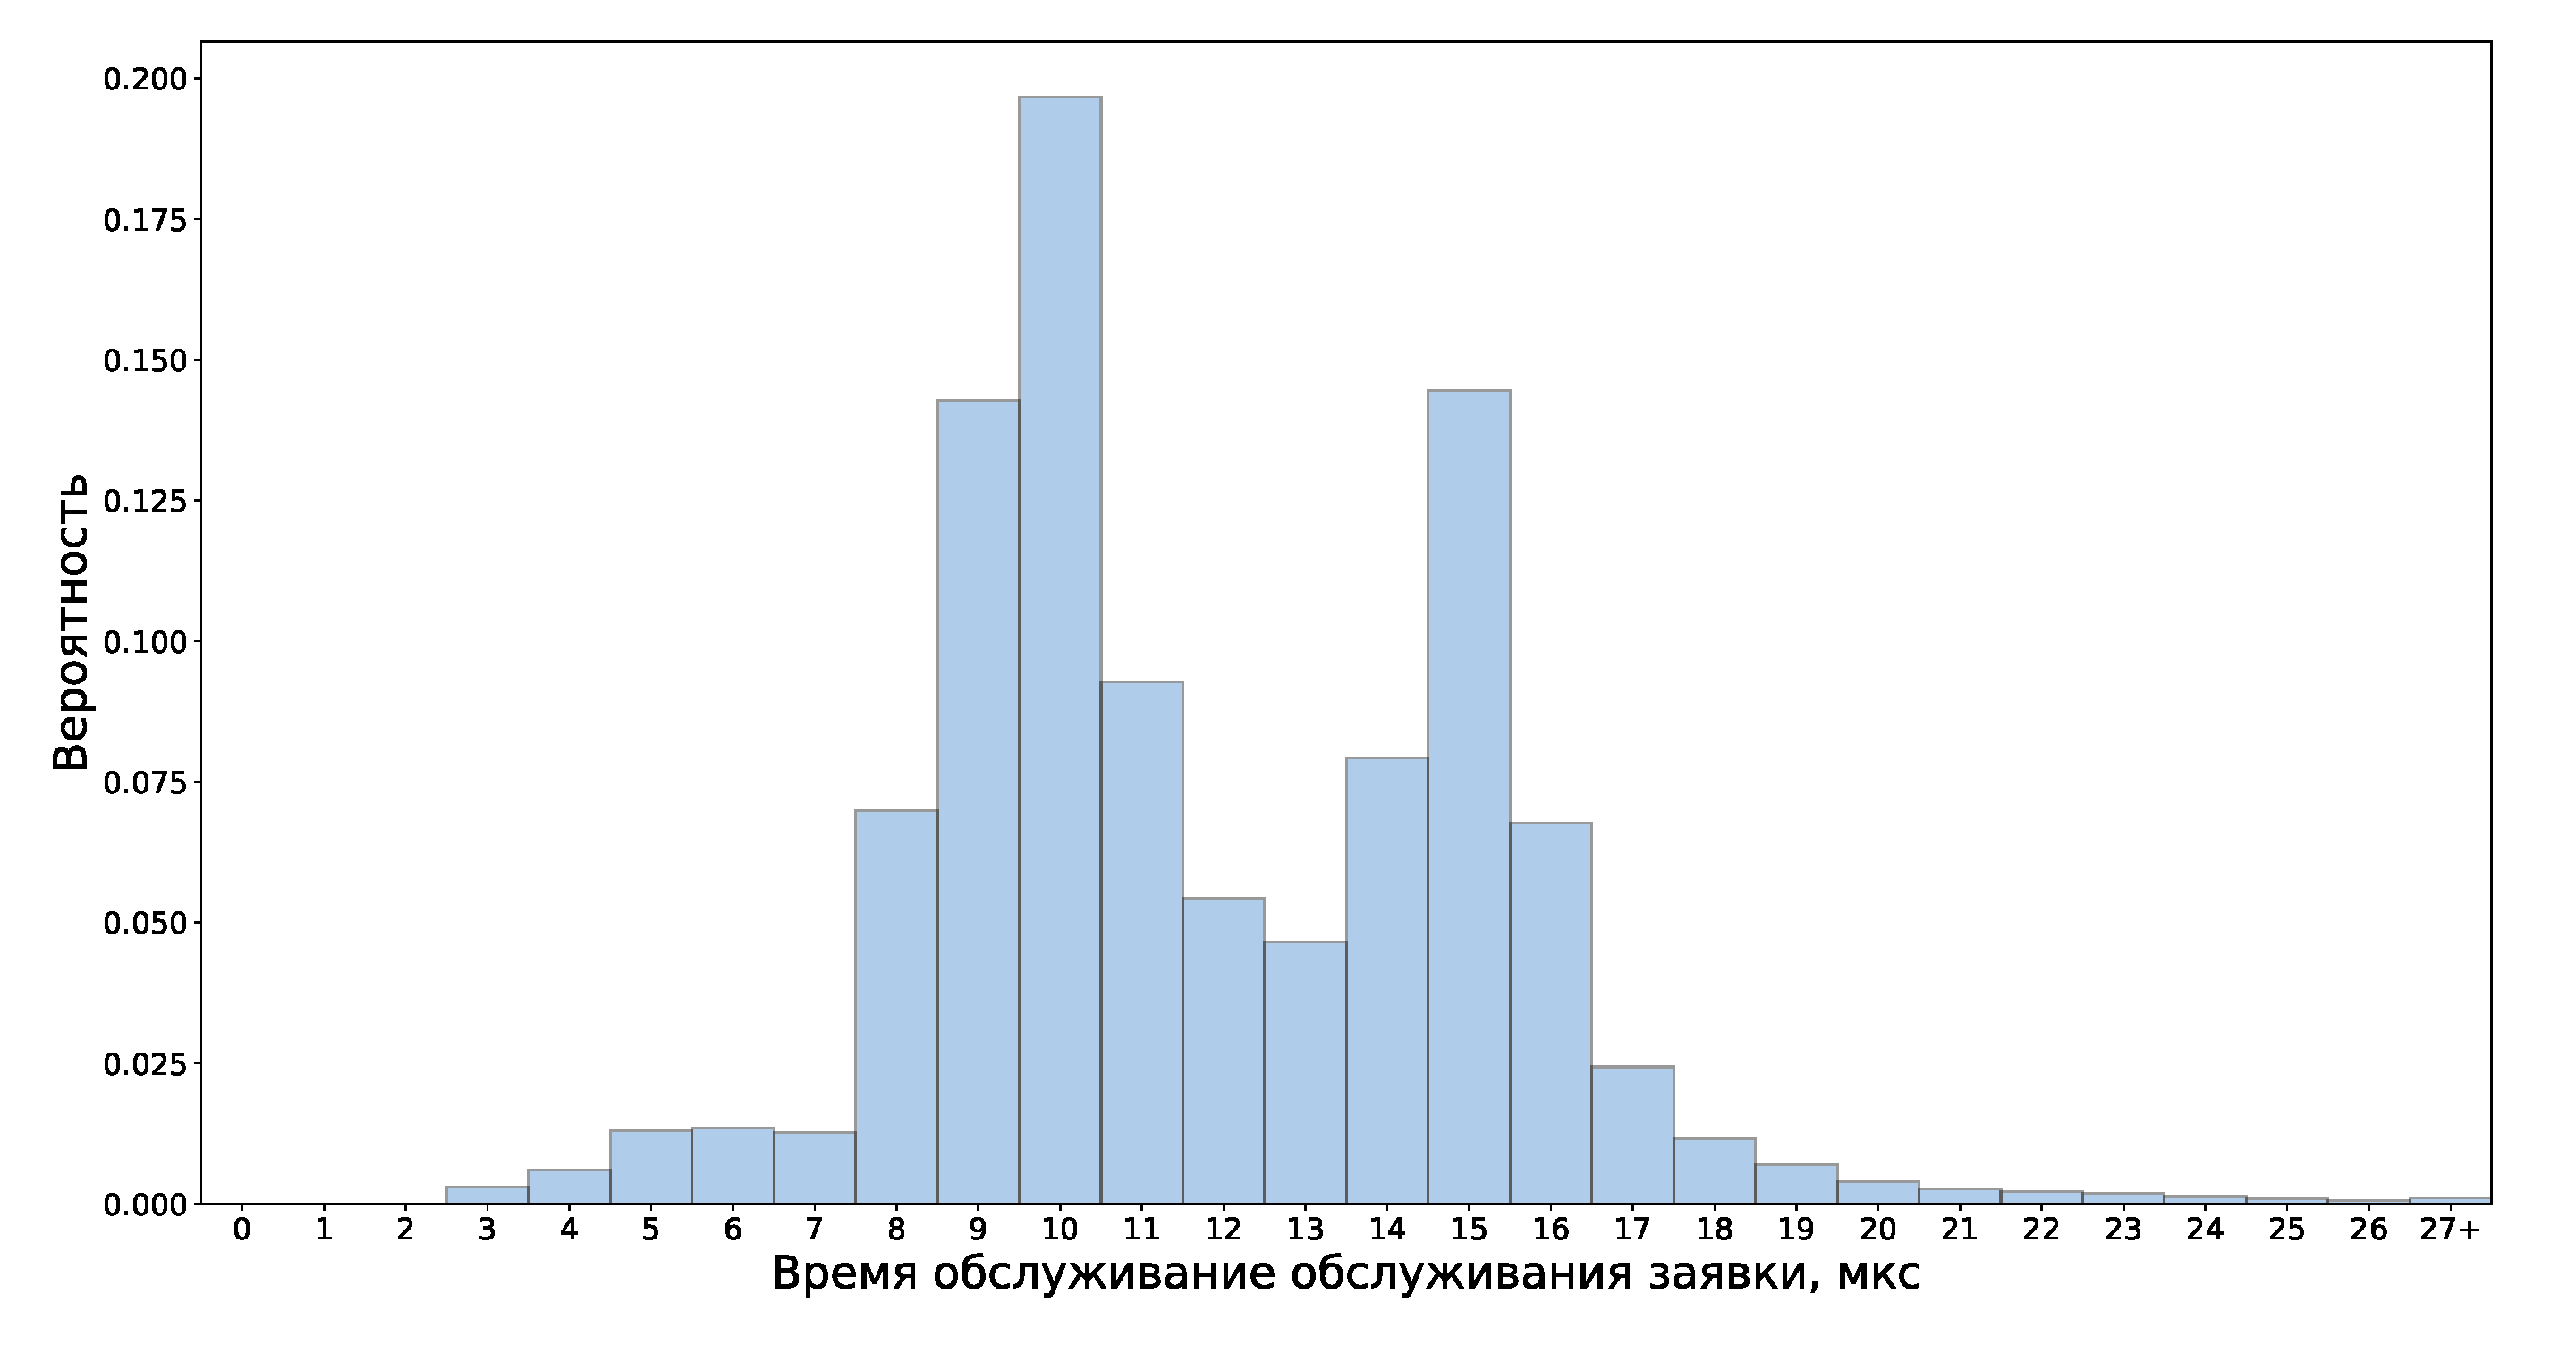
\includegraphics[width=\textwidth]{../../graphics/hist/Engine}
\end{figure}

\begin{table}[!h]
\caption{Процентили времени обслуживания заявок в процессе-обработчике}\label{chapter41:TableEngine}
\centering
\begin{tabular}{|l|l|l|l|l|l|l|l|}
\hline
Процентиль & 0\% & 50\% & 80\% & 90\% & 95\% & 99\% & 100\% \\ \hline
$T$, мкс & 2 & 11 & 15 & 16 & 17 & 21 & 285 \\ \hline
\end{tabular}
\end{table}

На рисунке \ref{chapter41:TRLatency} представлена гистограмма времени обслуживания заявок в процессе-шлюзе. В таблице \ref{chapter41:TableTR} представлены процентили времени обслуживания заявок в процессе-обработчике.
\begin{figure}[!h]
\caption{Гистограмма времени обслуживания заявки в процессе-шлюзе}
\label{chapter41:TRLatency}
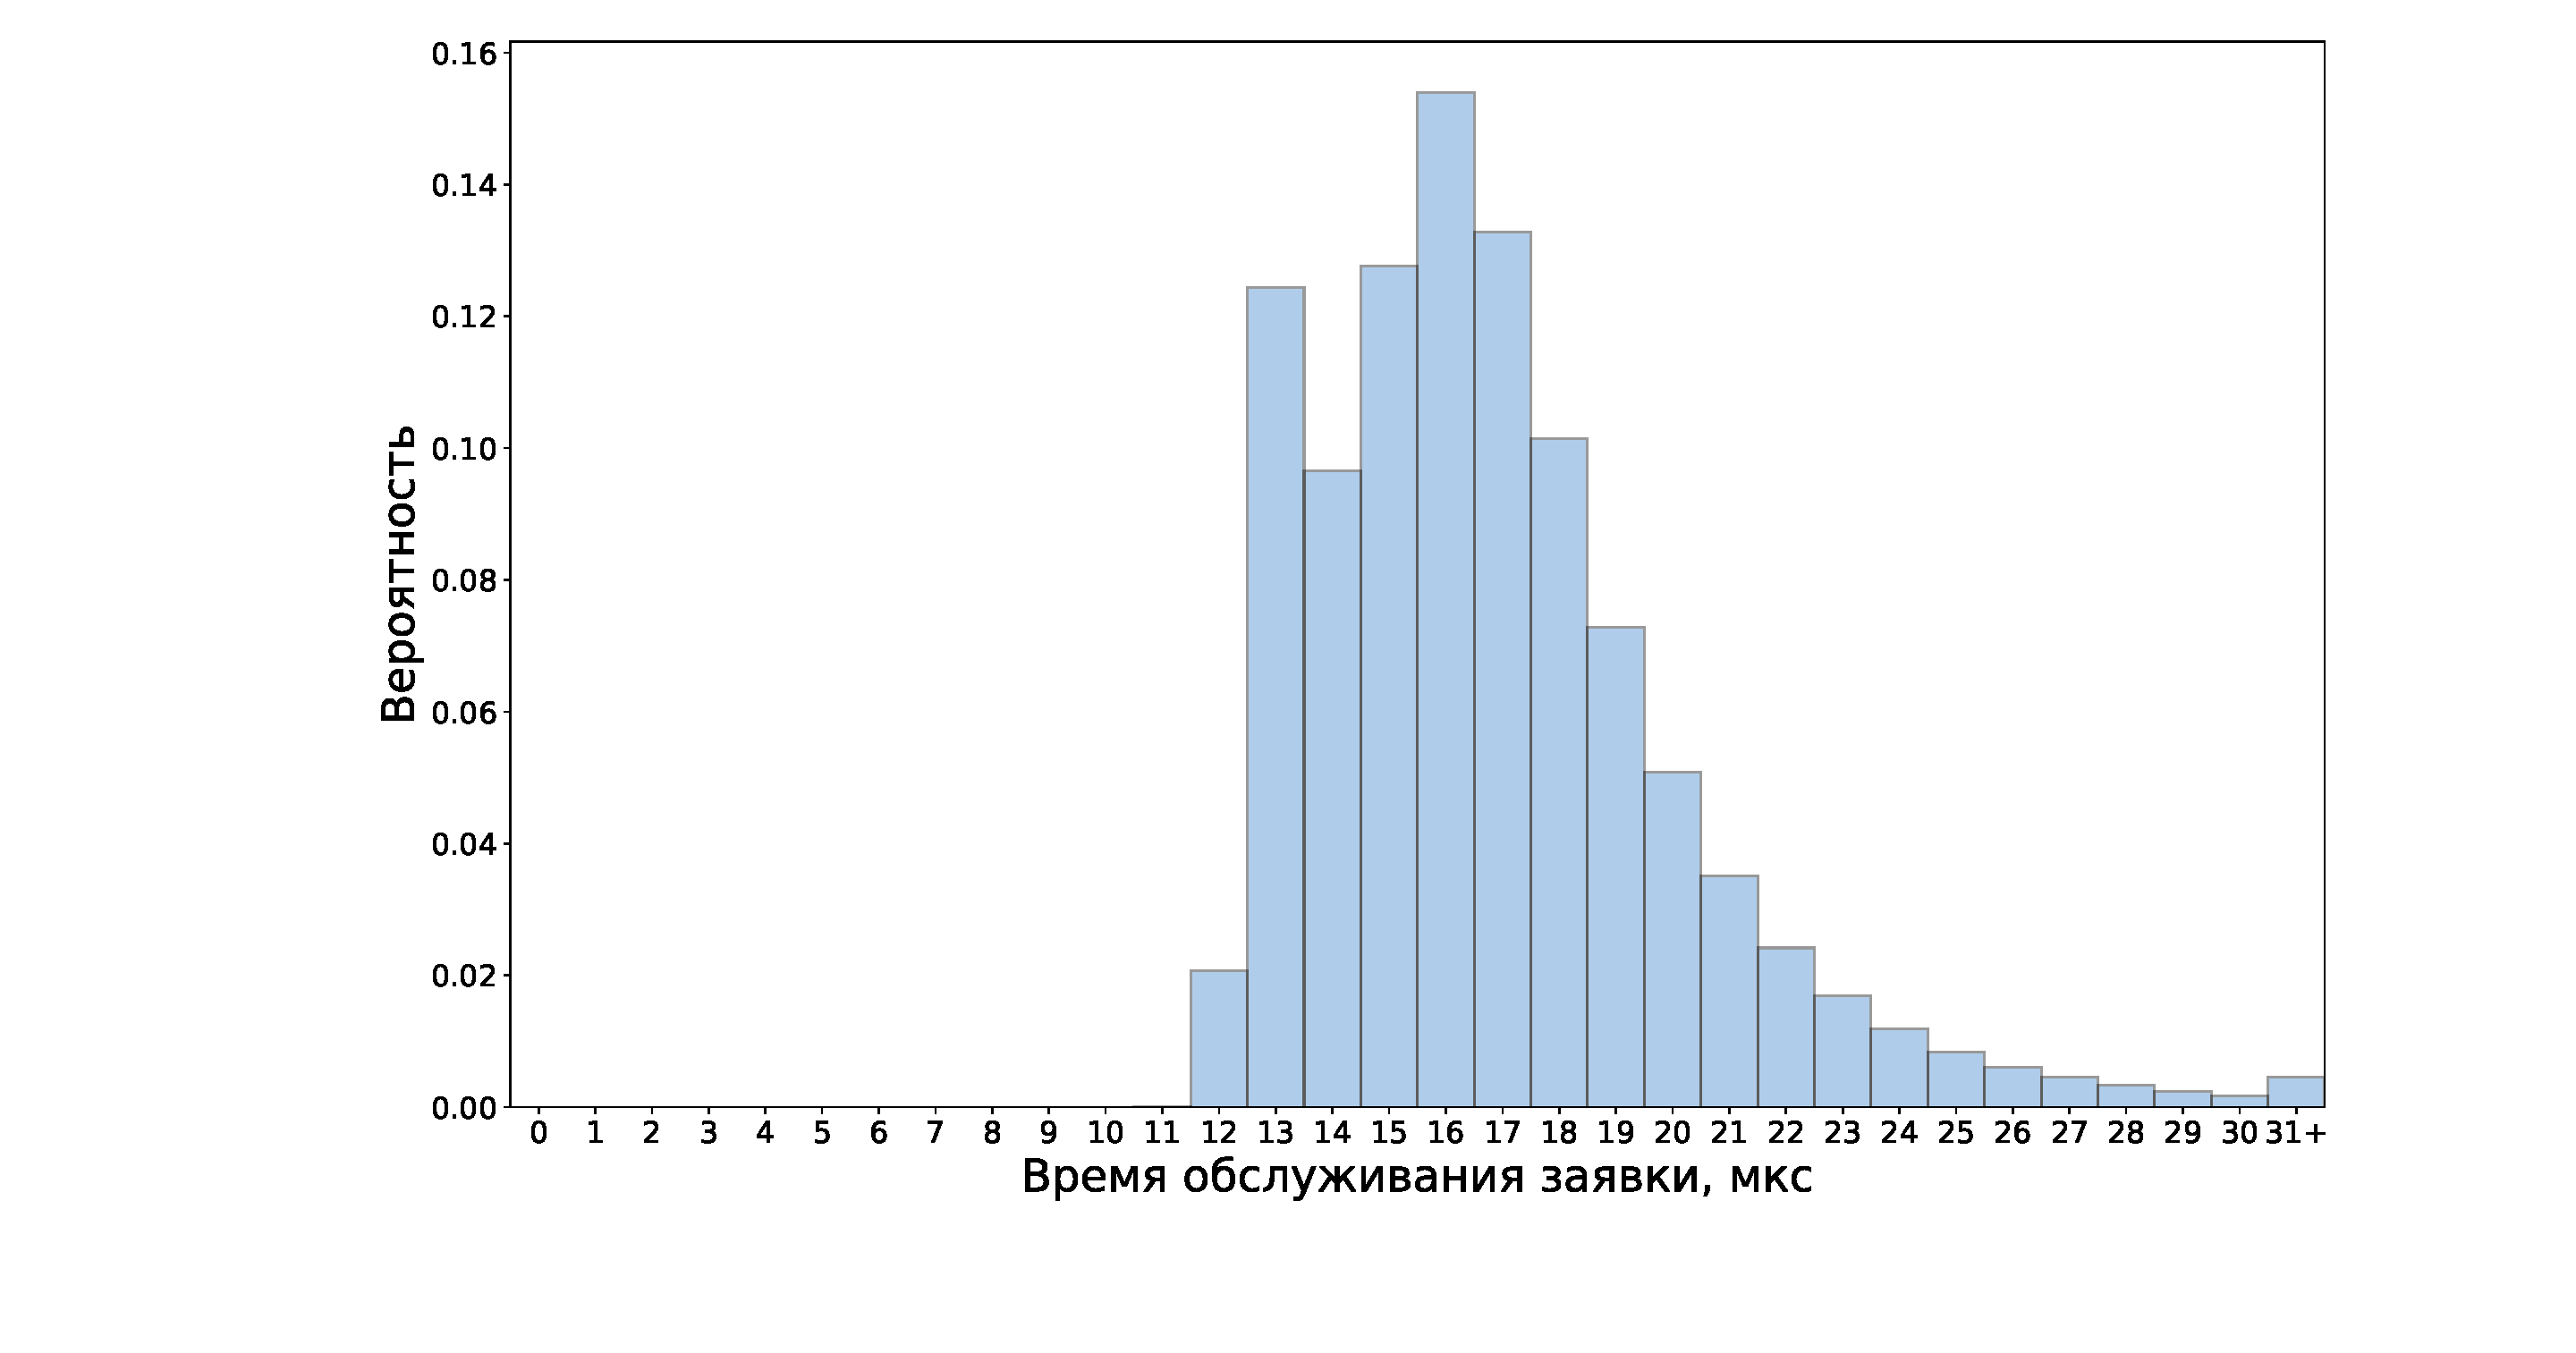
\includegraphics[width=\textwidth]{../../graphics/hist/TR}
\end{figure}

\begin{table}[!h]
\caption{Процентили времени обслуживания заявок в процессе-шлюзе}\label{chapter41:TableTR}
\centering
\begin{tabular}{|l|l|l|l|l|l|l|l|}
\hline
Процентиль & 0\% & 50\% & 80\% & 90\% & 95\% & 99\% & 100\% \\ \hline
$T$, мкс & 11 & 16 & 19 & 21 & 23 & 27 & 5678 \\ \hline
\end{tabular}
\end{table}

\textbf{TBD: а надо ли мне вообще говорить тогда про время обслуживания заявок в процессе-шлюзе? Может, убрать совсем?}
Как было сказано выше, в процессе-шлюзе заявки обслуживания вне транспортного потока, поэтому время обслуживания заявок в процессе-шлюзе не влияет на временную задержку на передачу данных. В случае с процессом-обработчиком значительная часть обслуживания заявки выполняется именно в транспортном потоке, что влияет на временную задержку на передачу данных, т.к. нахождение в очереди на обслуживание влияет на данный показатель.


\section{Использование TCP для передачи данных}


В качестве точки отсчета в настоящей работе выступает метод межпроцессного взаимодействия на основе TCP, используемый посредством сокетов \textbf{TBD: ссылка на определение и на раздел диссертации} \ref{chapter31:PureTCP}.

Показатели потока исходящих заявок из симулятора в данном эксперименте: $\Delta \in$ \textit{10 $\pm$ 4 мс}, $\delta \in$ \textit{50 $\pm$ 26 мкс}.

\begin{figure}[!h]
\caption{Гистограмма временной задержки на передачу данных между процессами при использовании TCP}
\label{chapter41:FigPureTCP}
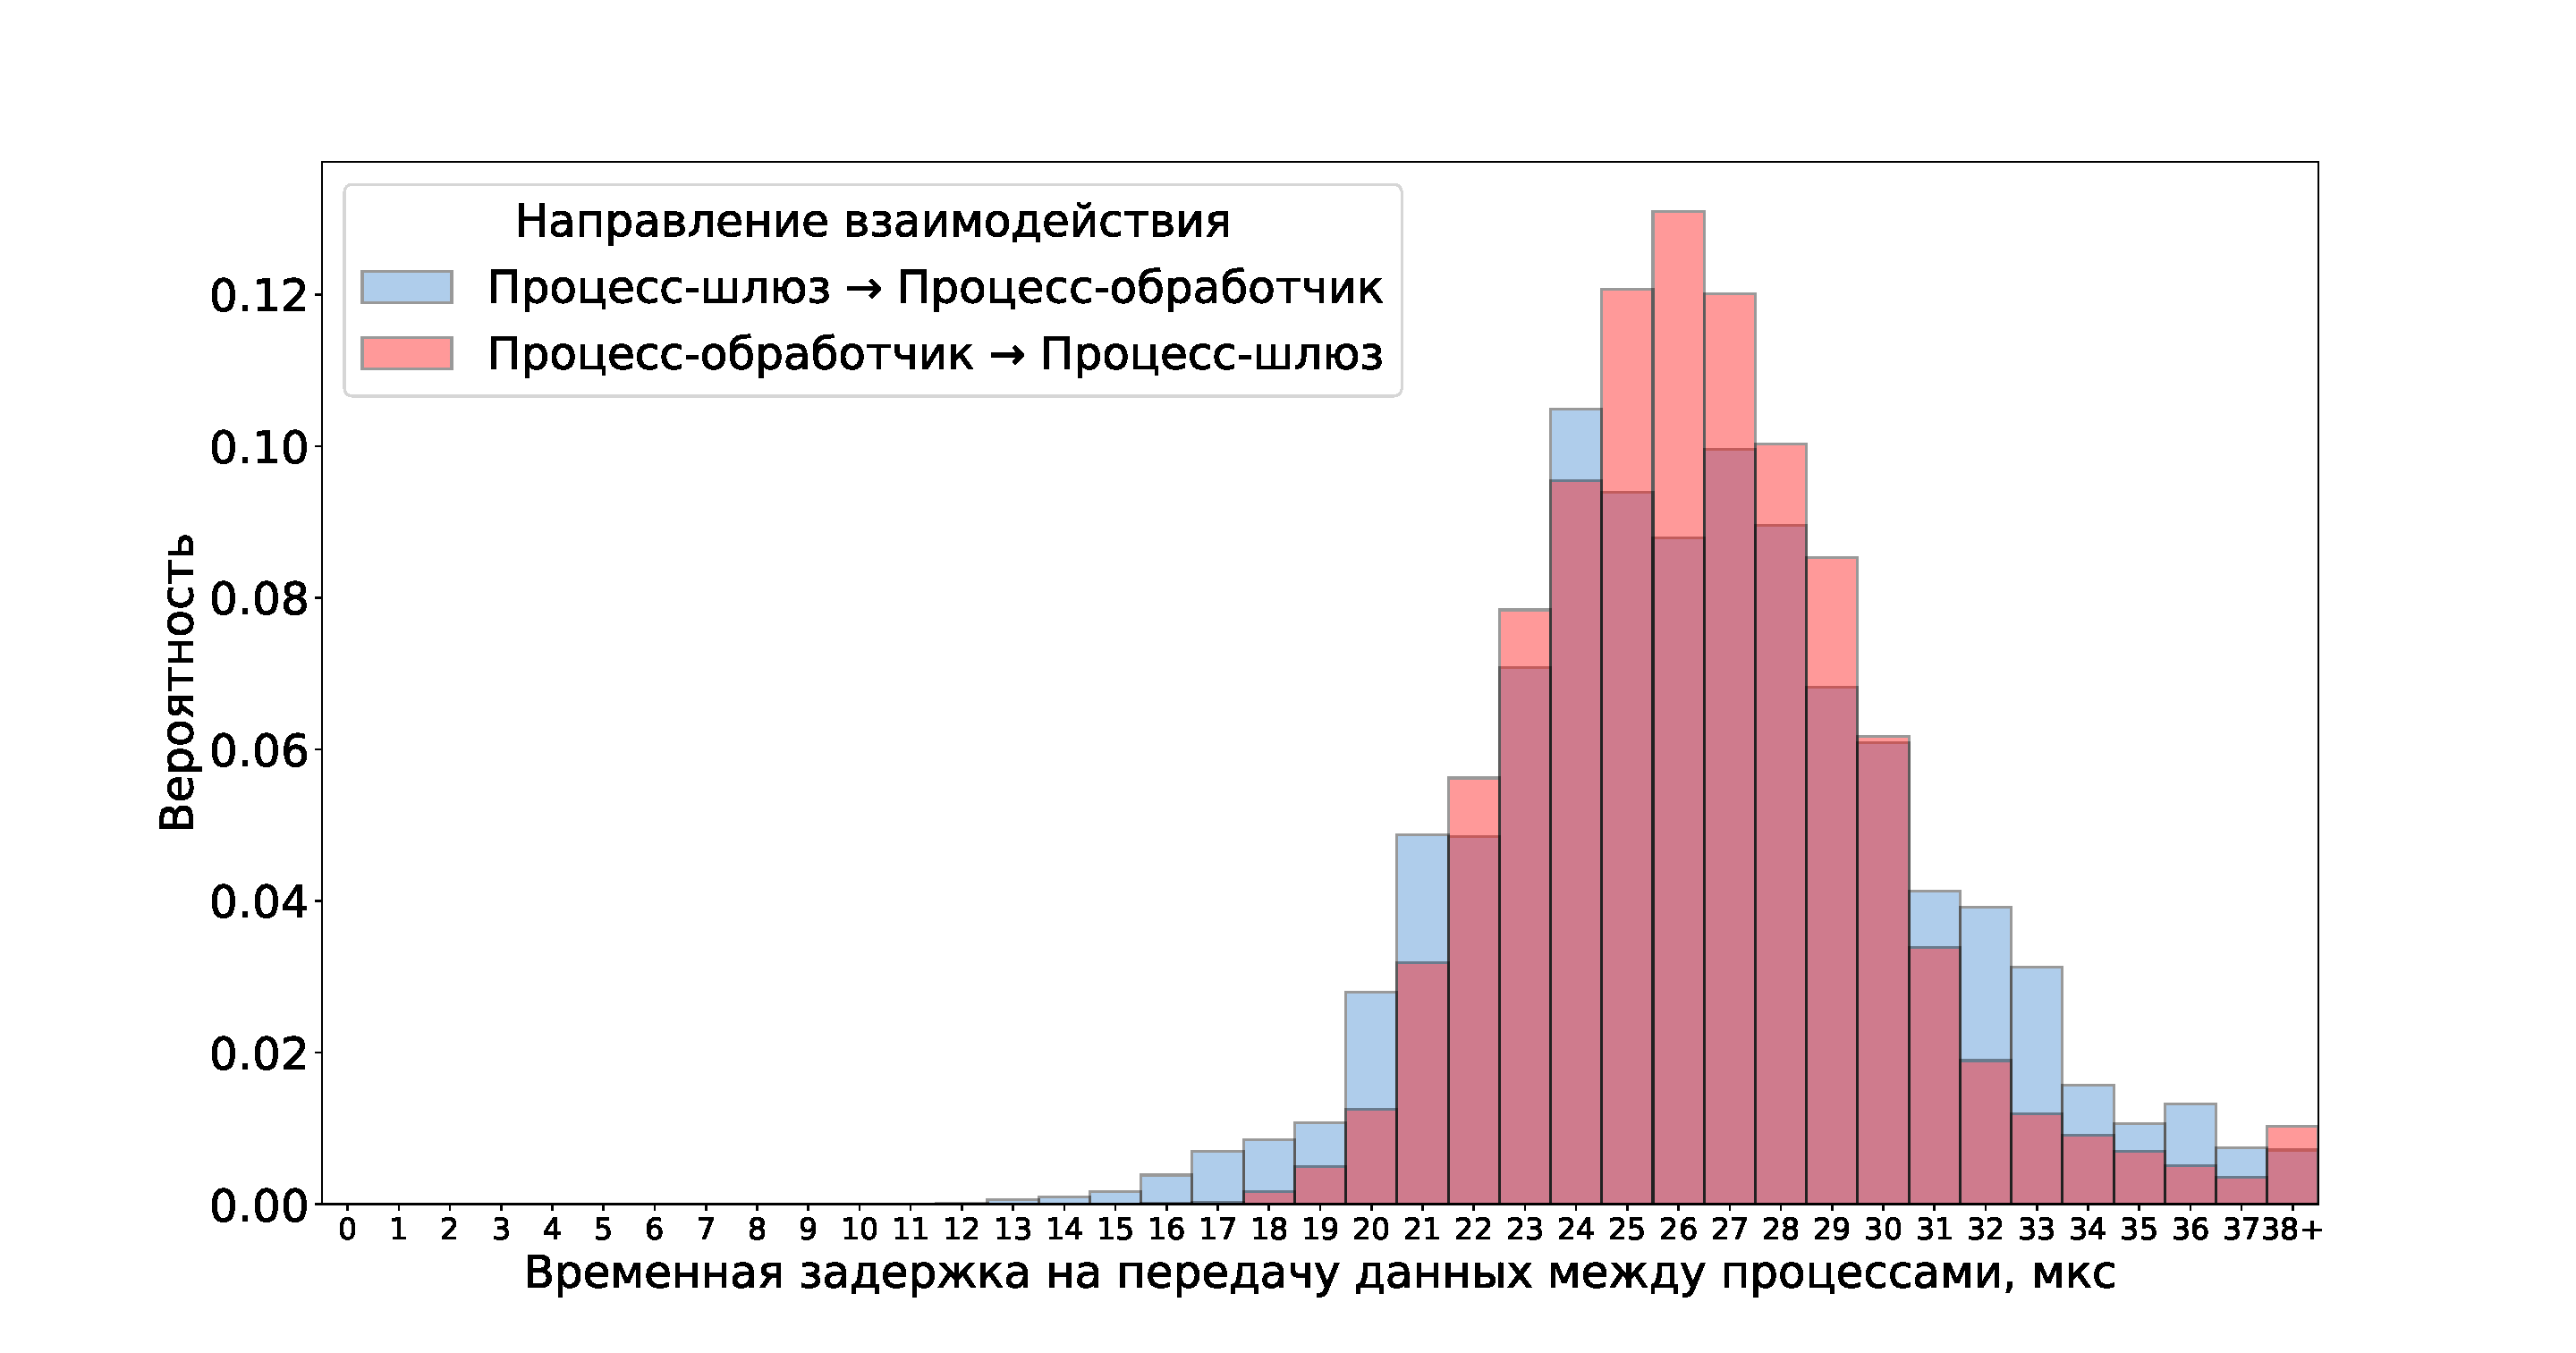
\includegraphics[width=\textwidth]{../../graphics/hist/PureTCP}
\end{figure}

Гистограмма временной задержки на передачу данных для данного метода приведена на Рисунке \ref{chapter41:FigPureTCP}. В Таблице \ref{chapter41:TablePureTCP} приведены основные временные характеристики данного метода.

\begin{table}[!h]
\caption{Основные показатели временной задержки на передачу данных для метода на основе TCP}\label{chapter41:TablePureTCP}
\centering
\begin{tabular}{|l|c|c|}
\hline
\begin{tabular}[c]{@{}l@{}}Направление\\ взаимодействия/\\ Показатель\end{tabular} & \multicolumn{1}{l|}{\begin{tabular}[c]{@{}l@{}}Процесс-шлюз $\rightarrow$\\ Процесс-обработчик\end{tabular}} & \multicolumn{1}{l|}{\begin{tabular}[c]{@{}l@{}}Процесс-обработчик $\rightarrow$\\ Процесс-шлюз\end{tabular}} \\ \hline
min(t), мкс & 9 & 13 \\ \hline
M(t), мкс & 27.5 $\pm$ 8.5 & 28 $\pm$ 7 \\ \hline
max(t), мс & 2.1 & 9.2 \\ \hline
\begin{tabular}[c]{@{}l@{}}$\Delta$, мс\end{tabular} & 10 $\pm$ 4 & 10 $\pm$ 4 \\ \hline
\begin{tabular}[c]{@{}l@{}}$\delta$, мкс\end{tabular} & 50 $\pm$ 26 & 87 $\pm$ 32 \\ \hline
\end{tabular}
\end{table}

Временная задержка на передачу данных в обоих направлениях имеет схожие значения. Это объясняется тем, что накладные расходы на использование TCP через механизм сокетов имеют подавляющее значение над прочими факторами, влияющими на межпроцессное взаимодействие.

\section{Использование разделяемой памяти для передачи данных}

\subsection{Использование TCP для оповещения о появлении данных}

Показатели потока исходящих заявок из симулятора в данном эксперименте: $\Delta \in$ \textit{10 $\pm$ 4 мс}, $\delta \in$ \textit{50 $\pm$ 27 мкс}.

В данном подразделе приведены данные об экспериментах с методом межпроцессного взаимодействия, описанным в Разделе \ref{chapter31:SignalTCP}.

\begin{figure}[!h]
\caption{Гистограмма временной задержки на передачу данных между процессами при использовании разделяемой памяти для передачи данных и TCP для оповещения о появлении данных в ней}
\label{chapter41:FigSignalTCP}
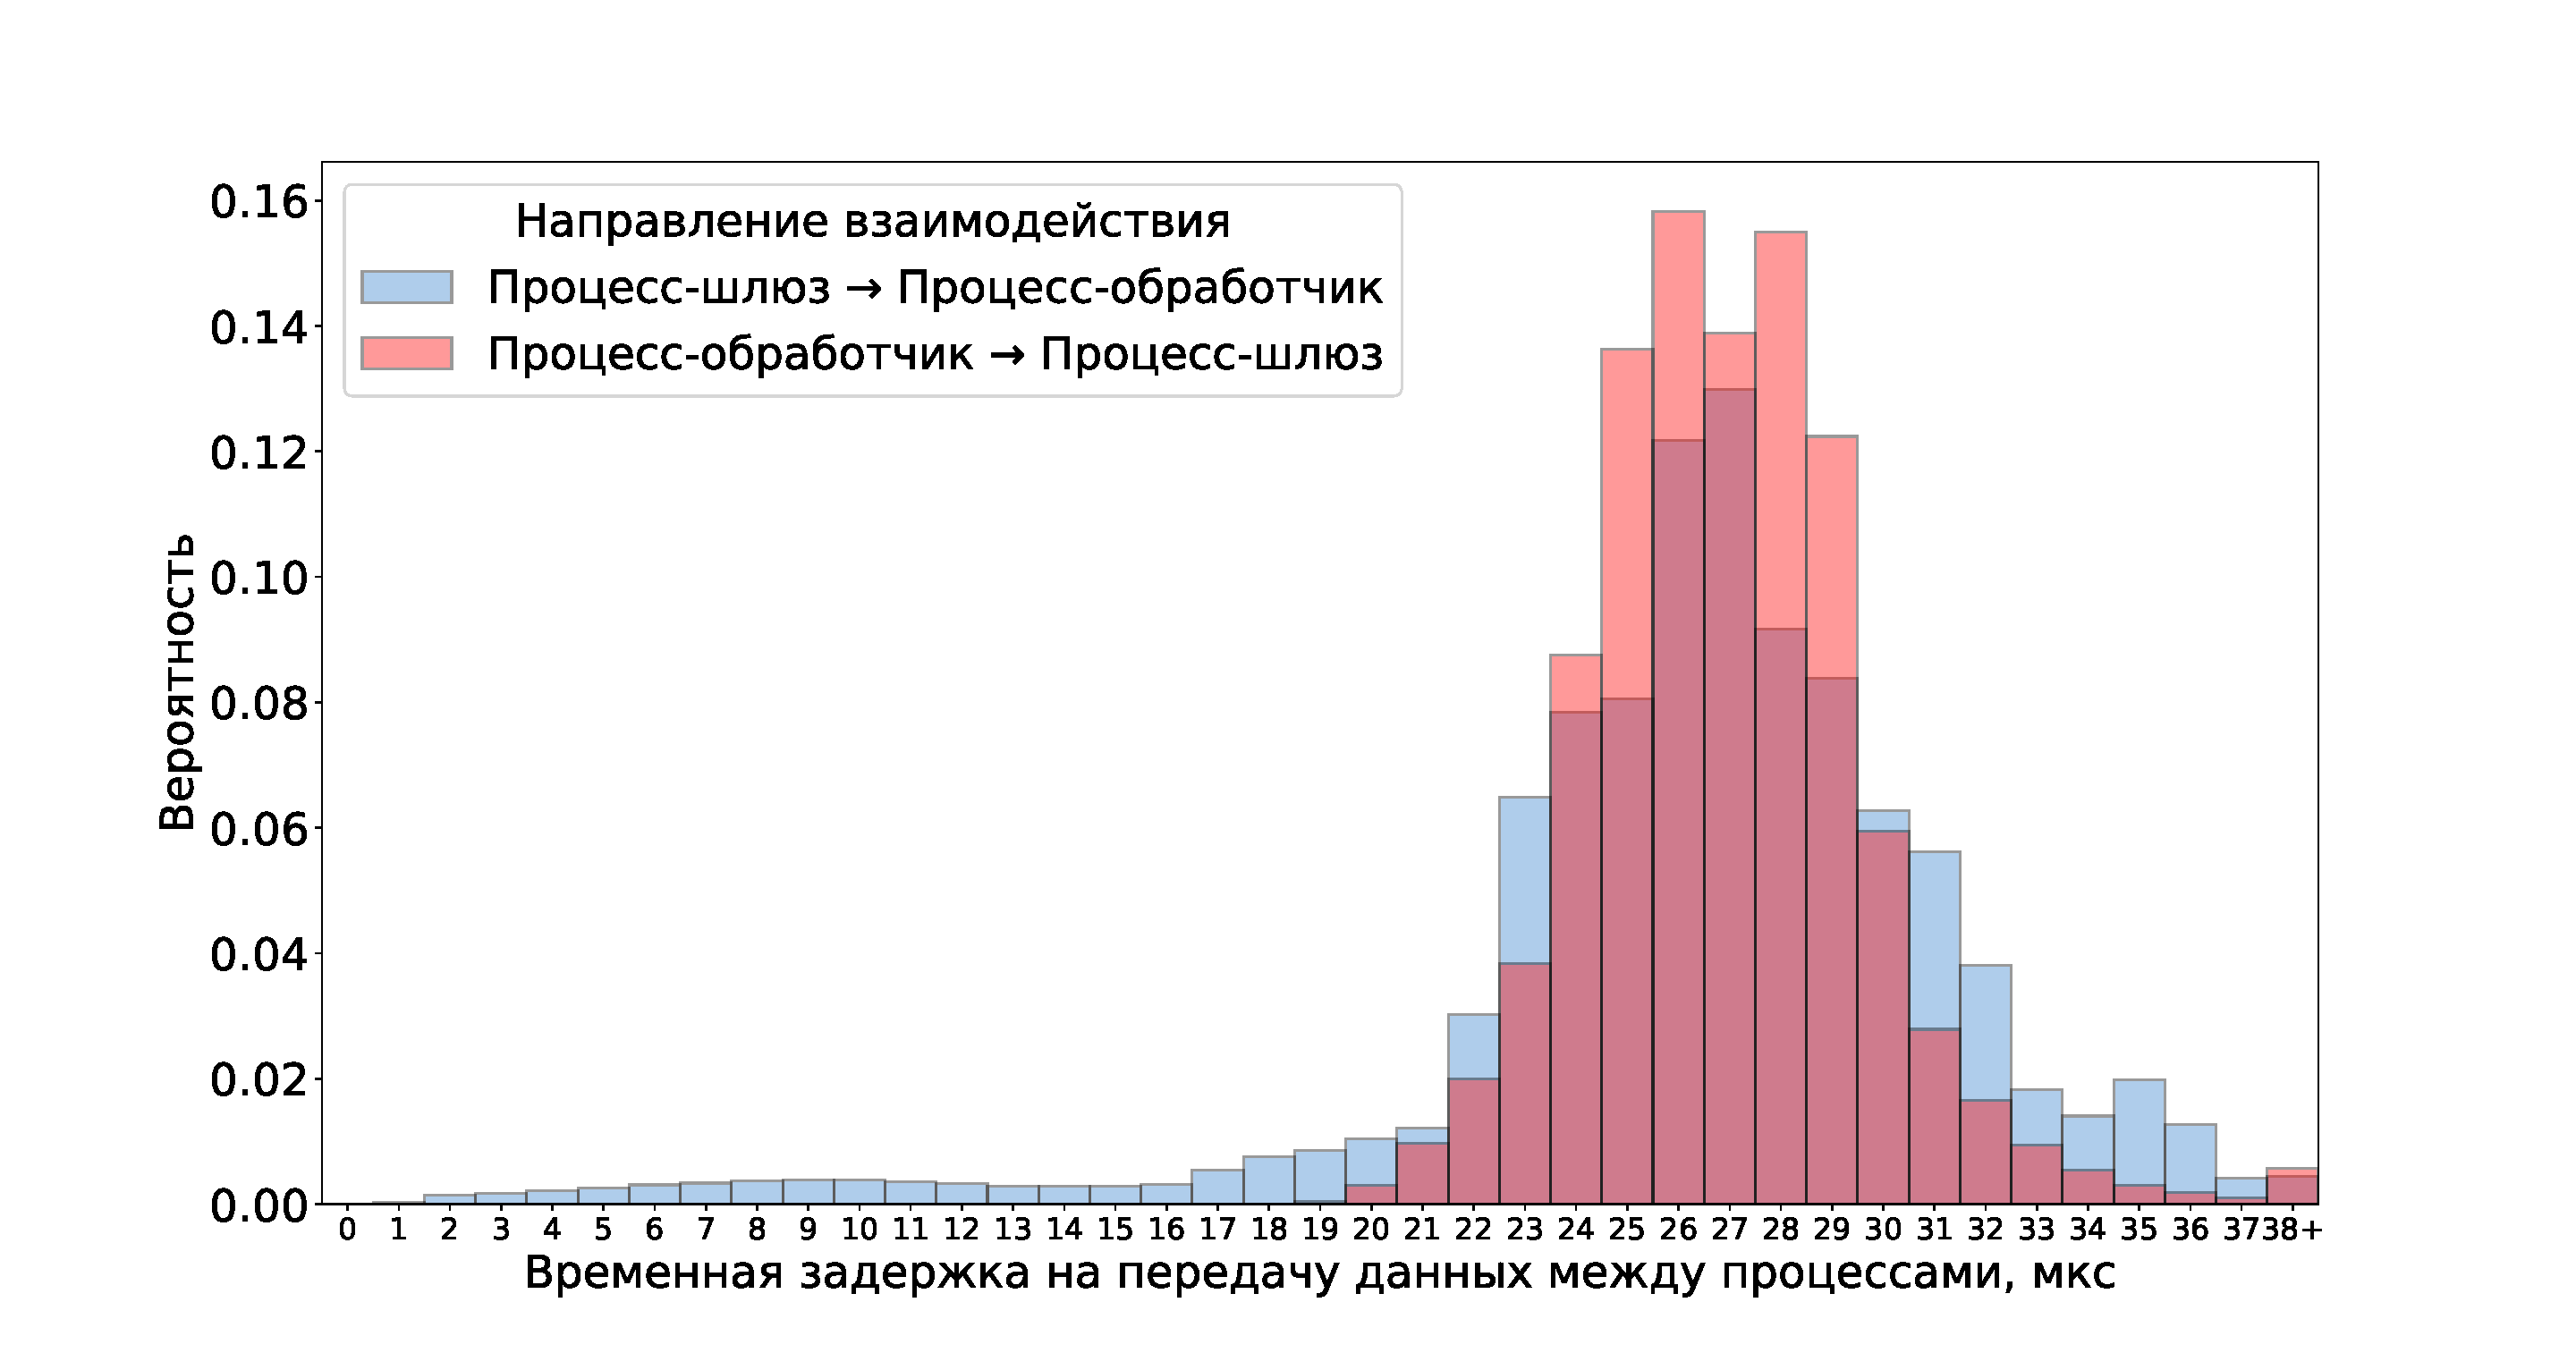
\includegraphics[width=\textwidth]{../../graphics/hist/SignalTCP}
\end{figure}

\begin{table}[!h]
\caption{Основные показатели временной задержки на передачу данных для метода, использующего разделяемую памяти для передачи данных и TCP для оповещения о появлении данных в ней}\label{chapter41:TableSignalTCP}
\centering
\begin{tabular}{|l|c|c|}
\hline
\begin{tabular}[c]{@{}l@{}}Направление\\ взаимодействия/\\ Показатель\end{tabular} & \multicolumn{1}{l|}{\begin{tabular}[c]{@{}l@{}}Процесс-шлюз $\rightarrow$\\ Процесс-обработчик\end{tabular}} & \multicolumn{1}{l|}{\begin{tabular}[c]{@{}l@{}}Процесс-обработчик $\rightarrow$\\ Процесс-шлюз\end{tabular}} \\ \hline
min(t), мкс & 1 & 3 \\ \hline
M(t), мкс & 22.5 $\pm$ 12.5 & 27.5 $\pm$ 5.5 \\ \hline
max(t), мс & 3 & 9.8 \\ \hline
\begin{tabular}[c]{@{}l@{}}$\Delta$, мс\end{tabular} & 10 $\pm$ 4 & 10 $\pm$ 4 \\ \hline
\begin{tabular}[c]{@{}l@{}}$\delta$, мкс\end{tabular} & 50 $\pm$ 27 & 87 $\pm$ 32 \\ \hline
\end{tabular}
\end{table}

В Таблице \ref{chapter41:TableSignalTCP} приведены основные временные характеристики данного метода. На Рисунке \ref{chapter41:FigSignalTCP} приведена гистограмма временной задержки на передачу данных для данного метода.

Как описано выше, значительная часть обслуживания заявки процессом-обработчиком происходит непосредственно в транспортном потоке. Из-за этого к моменту конца обработки текущей заявки очередная заявка уже может находиться в очереди в разделяемой памяти, что позволяет использовать оптимизацию, описанную в Разделе \ref{chapter31:SharedMemoryOptimization}. А именно принять и начать обслуживание очередной заявки, не используя дорогостоящий механизм оповещения, если заявка уже находится в очереди в разделяемой памяти. 

Прием заявки процессом-шлюзом не связан с обслуживанием заявки, поэтому к моменту, когда процесс-шлюз заканчивает прием и диспетчеризацию заявки, очередь входящих заявок в данном эксперименте пуста и поток-шлюз переходит к пассивному ожиданию новых заявок. Таким образом, приему и обслуживанию большинства заявок сопутствует пассивное ожидание сигнала по TCP, что негативно сказывается на временной задержке на передачу данных.

\subsection{Использование мультиплексора в разделяемой памяти для оповещения о появлении данных}

В данном подразделе приведены данные об экспериментах с семейством методов межпроцессного взаимодействия, описанными в Разделе \ref{chapter31:Mux}.

\subsubsection{Блокирующие методы}

В блокирующих методах поток мультиплексора событий использует примитив \textit{futex} 
\textbf{TBD:Может, сослаться на определение futex?}
для пассивного ожидания новых сигналов (см. Разделы \ref{chapter31:BlockingHSHA} и \ref{chapter31:BlockingLF}).

\paragraph{Диспетчеризация и обработка соединений по модели "Полусинхронный/Полуреактивный"}

Показатели потока исходящих заявок из симулятора в данном эксперименте: $\Delta \in$ \textit{10 $\pm$ 4 мс}, $\delta \in$ \textit{51 $\pm$ 28 мкс}.

В данном подразделе приведены данные об экспериментах с методом межпроцессного взаимодействия, описанным в Разделе \ref{chapter31:BlockingHSHA}.

\begin{figure}[!h]
\caption{Гистограмма временной задержки на передачу данных между процессами для метода, использующего разделяемую память для передачи данных, блокирующий мультиплексор в разделяемой памяти и метод ''Полусинхронный/Полуреактивный`` при обслуживании заявок}
\label{chapter41:FigBlockingHSHA}
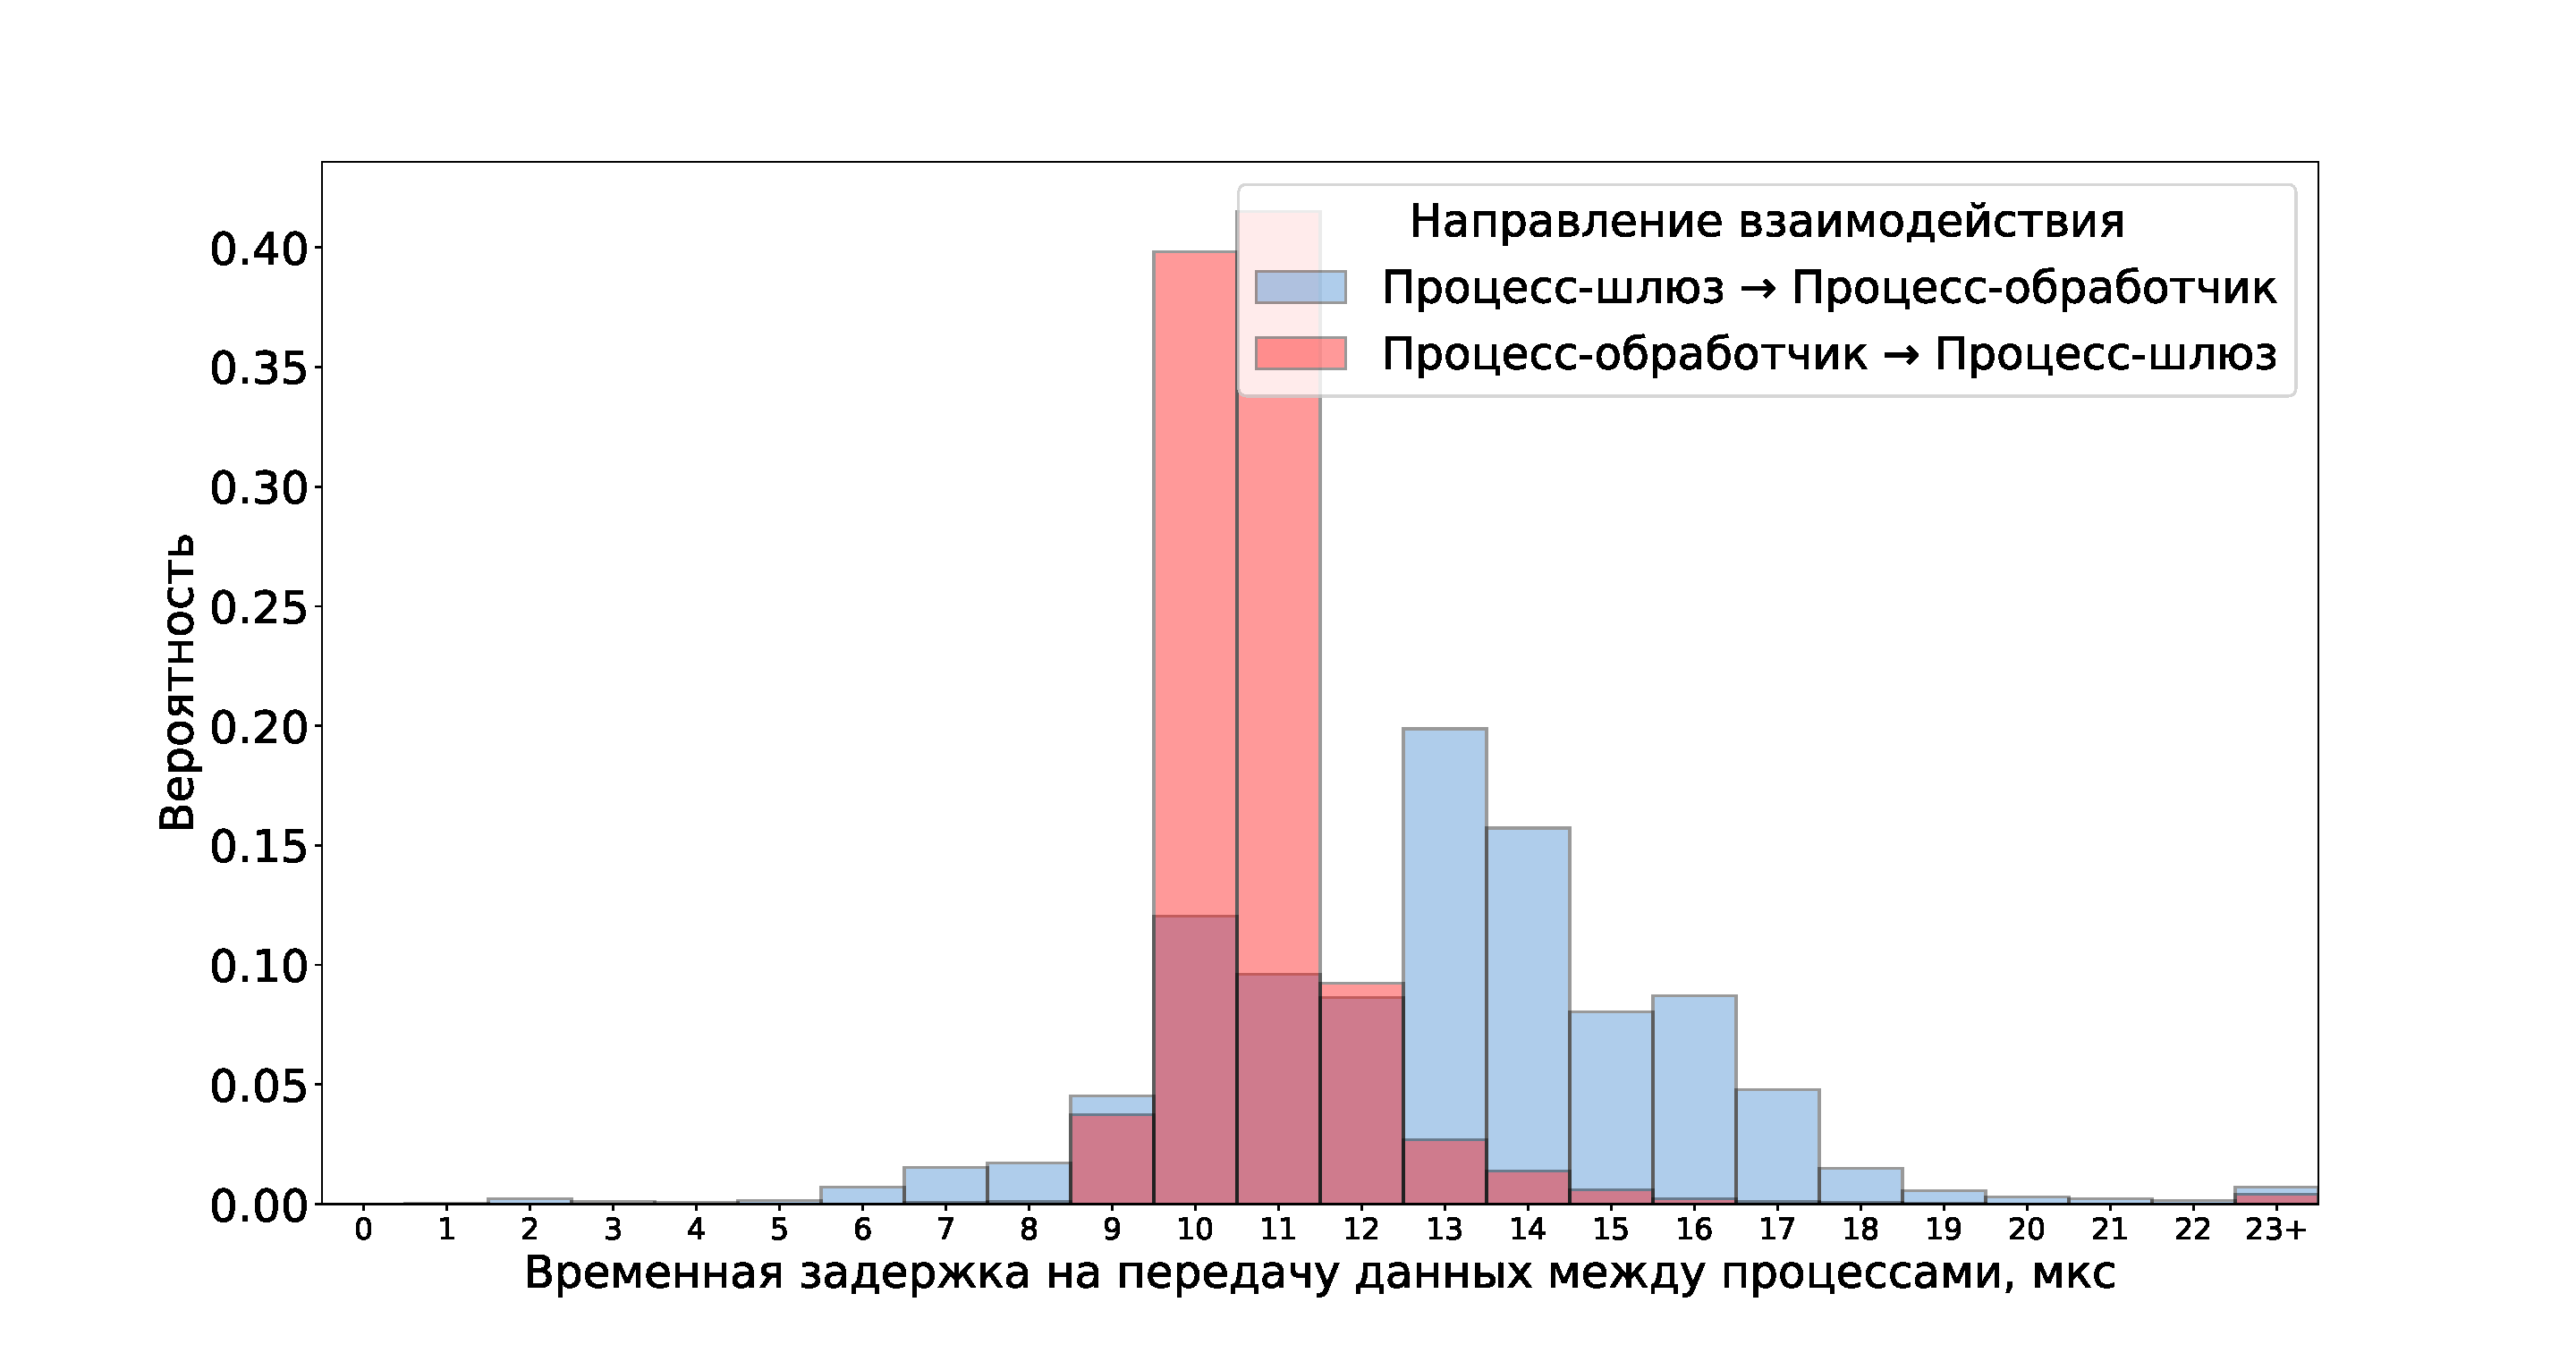
\includegraphics[width=\textwidth]{../../graphics/hist/BlockingHSHA}
\end{figure}

\begin{table}[!h]
\caption{Основные показатели временной задержки на передачу данных между процессами для метода, использующего разделяемую память для передачи данных, блокирующий мультиплексор в разделяемой памяти и метод ''Полусинхронный/Полуреактивный`` при обслуживании заявок}\label{chapter41:TableBlockingHSHA}
\centering
\begin{tabular}{|l|c|c|}
\hline
\begin{tabular}[c]{@{}l@{}}Направление\\ взаимодействия/\\ Показатель\end{tabular} & \multicolumn{1}{l|}{\begin{tabular}[c]{@{}l@{}}Процесс-шлюз $\rightarrow$\\ Процесс-обработчик\end{tabular}} & \multicolumn{1}{l|}{\begin{tabular}[c]{@{}l@{}}Процесс-обработчик $\rightarrow$\\ Процесс-шлюз\end{tabular}} \\ \hline
min(t), мкс & 1 & 3 \\ \hline
M(t) $\pm$ 95\%, мкс & 12.5 $\pm$ 5.5 & 11.5 $\pm$ 2.5 \\ \hline
max(t), мс & 6.9 & 11.6 \\ \hline
\begin{tabular}[c]{@{}l@{}}$\Delta$, мс\end{tabular} & 10 $\pm$ 4 & 10 $\pm$ 4 \\ \hline
\begin{tabular}[c]{@{}l@{}}$\delta$, мкс\end{tabular} & 51 $\pm$ 28 & 91 $\pm$ 36 \\ \hline
\end{tabular}
\end{table}

В Таблице \ref{chapter41:TableBlockingHSHA} приведены основные временные характеристики данного метода. На Рисунке \ref{chapter41:FigBlockingHSHA} приведена гистограмма временной задержки на передачу данных для данного метода.

Использовании более эффективного метода межпроцессного взаимодействия наглядно показывает эффект от влияния времени обслуживания заявки в транспортном потоке на временную задержку на передачу данных. Процесс-шлюз с минимальной временной задержкой принимает и диспетчеризует заявку для дальнейшей обработки и сразу же готов принимать следующую заявку. Процесс-обработчик же использует транспортный поток для частичного обслуживания заявки (см. Рисунок \ref{chapter41:EngineLatency}), а потому в среднем временная задержка на передачу данных имеет худшие показатели, так как это может задерживать прием очередных заявок.

\paragraph{Диспетчеризация и обработка соединений по модели "Лидер/Последователи"}

Показатели потока исходящих заявок из симулятора в данном эксперименте: $\Delta \in$ \textit{8.4 $\pm$ 5.3 мс}, $\delta \in$ \textit{52 $\pm$ 28 мкс}.

В данном подразделе приведены данные об экспериментах с методом межпроцессного взаимодействия, описанным в Разделе \ref{chapter31:BlockingLF}.

В Таблице \ref{chapter41:TableBlockingLF} приведены основные временные характеристики данного метода. \textbf{TBD}

На Рисунке \ref{chapter41:FigBlockingLF} приведена гистограмма временной задержки на передачу данных для данного метода.

\begin{figure}[!h]
\caption{Гистограмма временной задержки на передачу данных между процессами для метода, использующего разделяемую память для передачи данных, блокирующий мультиплексор в разделяемой памяти и метод ''Лидер/Последователи`` при обслуживании заявок}
\label{chapter41:FigBlockingLF}
\includegraphics[width=\textwidth]{../../graphics/hist/BlockingLF}
\end{figure}

\begin{table}[!h]
\caption{Основные показатели временной задержки на передачу данных между процессами для метода, использующего разделяемую память для передачи данных, блокирующий мультиплексор в разделяемой памяти и метод ''Лидер/Последователи`` при обслуживании заявок}\label{chapter41:TableBlockingLF}
\centering
\begin{tabular}{|l|c|c|}
\hline
\begin{tabular}[c]{@{}l@{}}Направление\\ взаимодействия/\\ Показатель\end{tabular} & \multicolumn{1}{l|}{\begin{tabular}[c]{@{}l@{}}Процесс-шлюз $\rightarrow$\\ Процесс-обработчик\end{tabular}} & \multicolumn{1}{l|}{\begin{tabular}[c]{@{}l@{}}Процесс-обработчик $\rightarrow$\\ Процесс-шлюз\end{tabular}} \\ \hline
min(t), мкс & 1 & 2 \\ \hline
M(t) $\pm$ 95\%, мкс & 11.5 $\pm$ 6.5 & 9.5 $\pm$ 1.5 \\ \hline
max(t), мс & 2.4 & 9.5 \\ \hline
\begin{tabular}[c]{@{}l@{}}$\Delta$, мс\end{tabular} & 8.4 $\pm$ 5.3 & 8.4 $\pm$ 5.3 \\ \hline
\begin{tabular}[c]{@{}l@{}}$\delta$, мкс\end{tabular} & 52 $\pm$ 29 & 90 $\pm$ 35 \\ \hline
\end{tabular}
\end{table}

Аналогичный эффект как при использовании предыдущего метода наблюдается и при использовании метода ''Лидер/Последователи``. Отличие состоит в меньшей временной задержке на передачу данных в пределах 1-2 мкс.

\subsubsection{Неблокирующий метод}

В неблокирующем методе поток мультиплексора событий метод активного ожидания новых сигналов (см. Раздел \ref{chapter31:NonBlockingLF}). В данном параграфе рассматривается исключительно метод обслуживания заявок ''Лидер/Последователи`` т.к. в параграфе выше она показала лучший результат по сравнению с методом обслуживания заявок ''Полусинхронный/Полуреактивный``.

\paragraph{Диспетчеризация и обработка соединений по модели "Лидер/Последователи"}

Показатели потока исходящих заявок из симулятора в данном эксперименте: $\Delta \in$ \textit{7.1 $\pm$ 5.8 мс}, $\delta \in$ \textit{83 $\pm$ 61 мкс}.

В данном подразделе приведены данные об экспериментах с методом межпроцессного взаимодействия, описанным в Разделе \ref{chapter31:NonBlockingLF}.

В Таблице \ref{chapter41:TableNonBlockingLF} приведены основные временные характеристики данного метода. На Рисунке \ref{chapter41:FigNonBlockingLF} приведена гистограмма временной задержки на передачу данных для данного метода.

\begin{figure}[!h]
\caption{Гистограмма временной задержки на передачу данных между процессами для метода, использующего разделяемую память для передачи данных, неблокирующий мультиплексор в разделяемой памяти и модель ''Лидер/Последователи`` при обслуживании заявок}
\label{chapter41:FigNonBlockingLF}
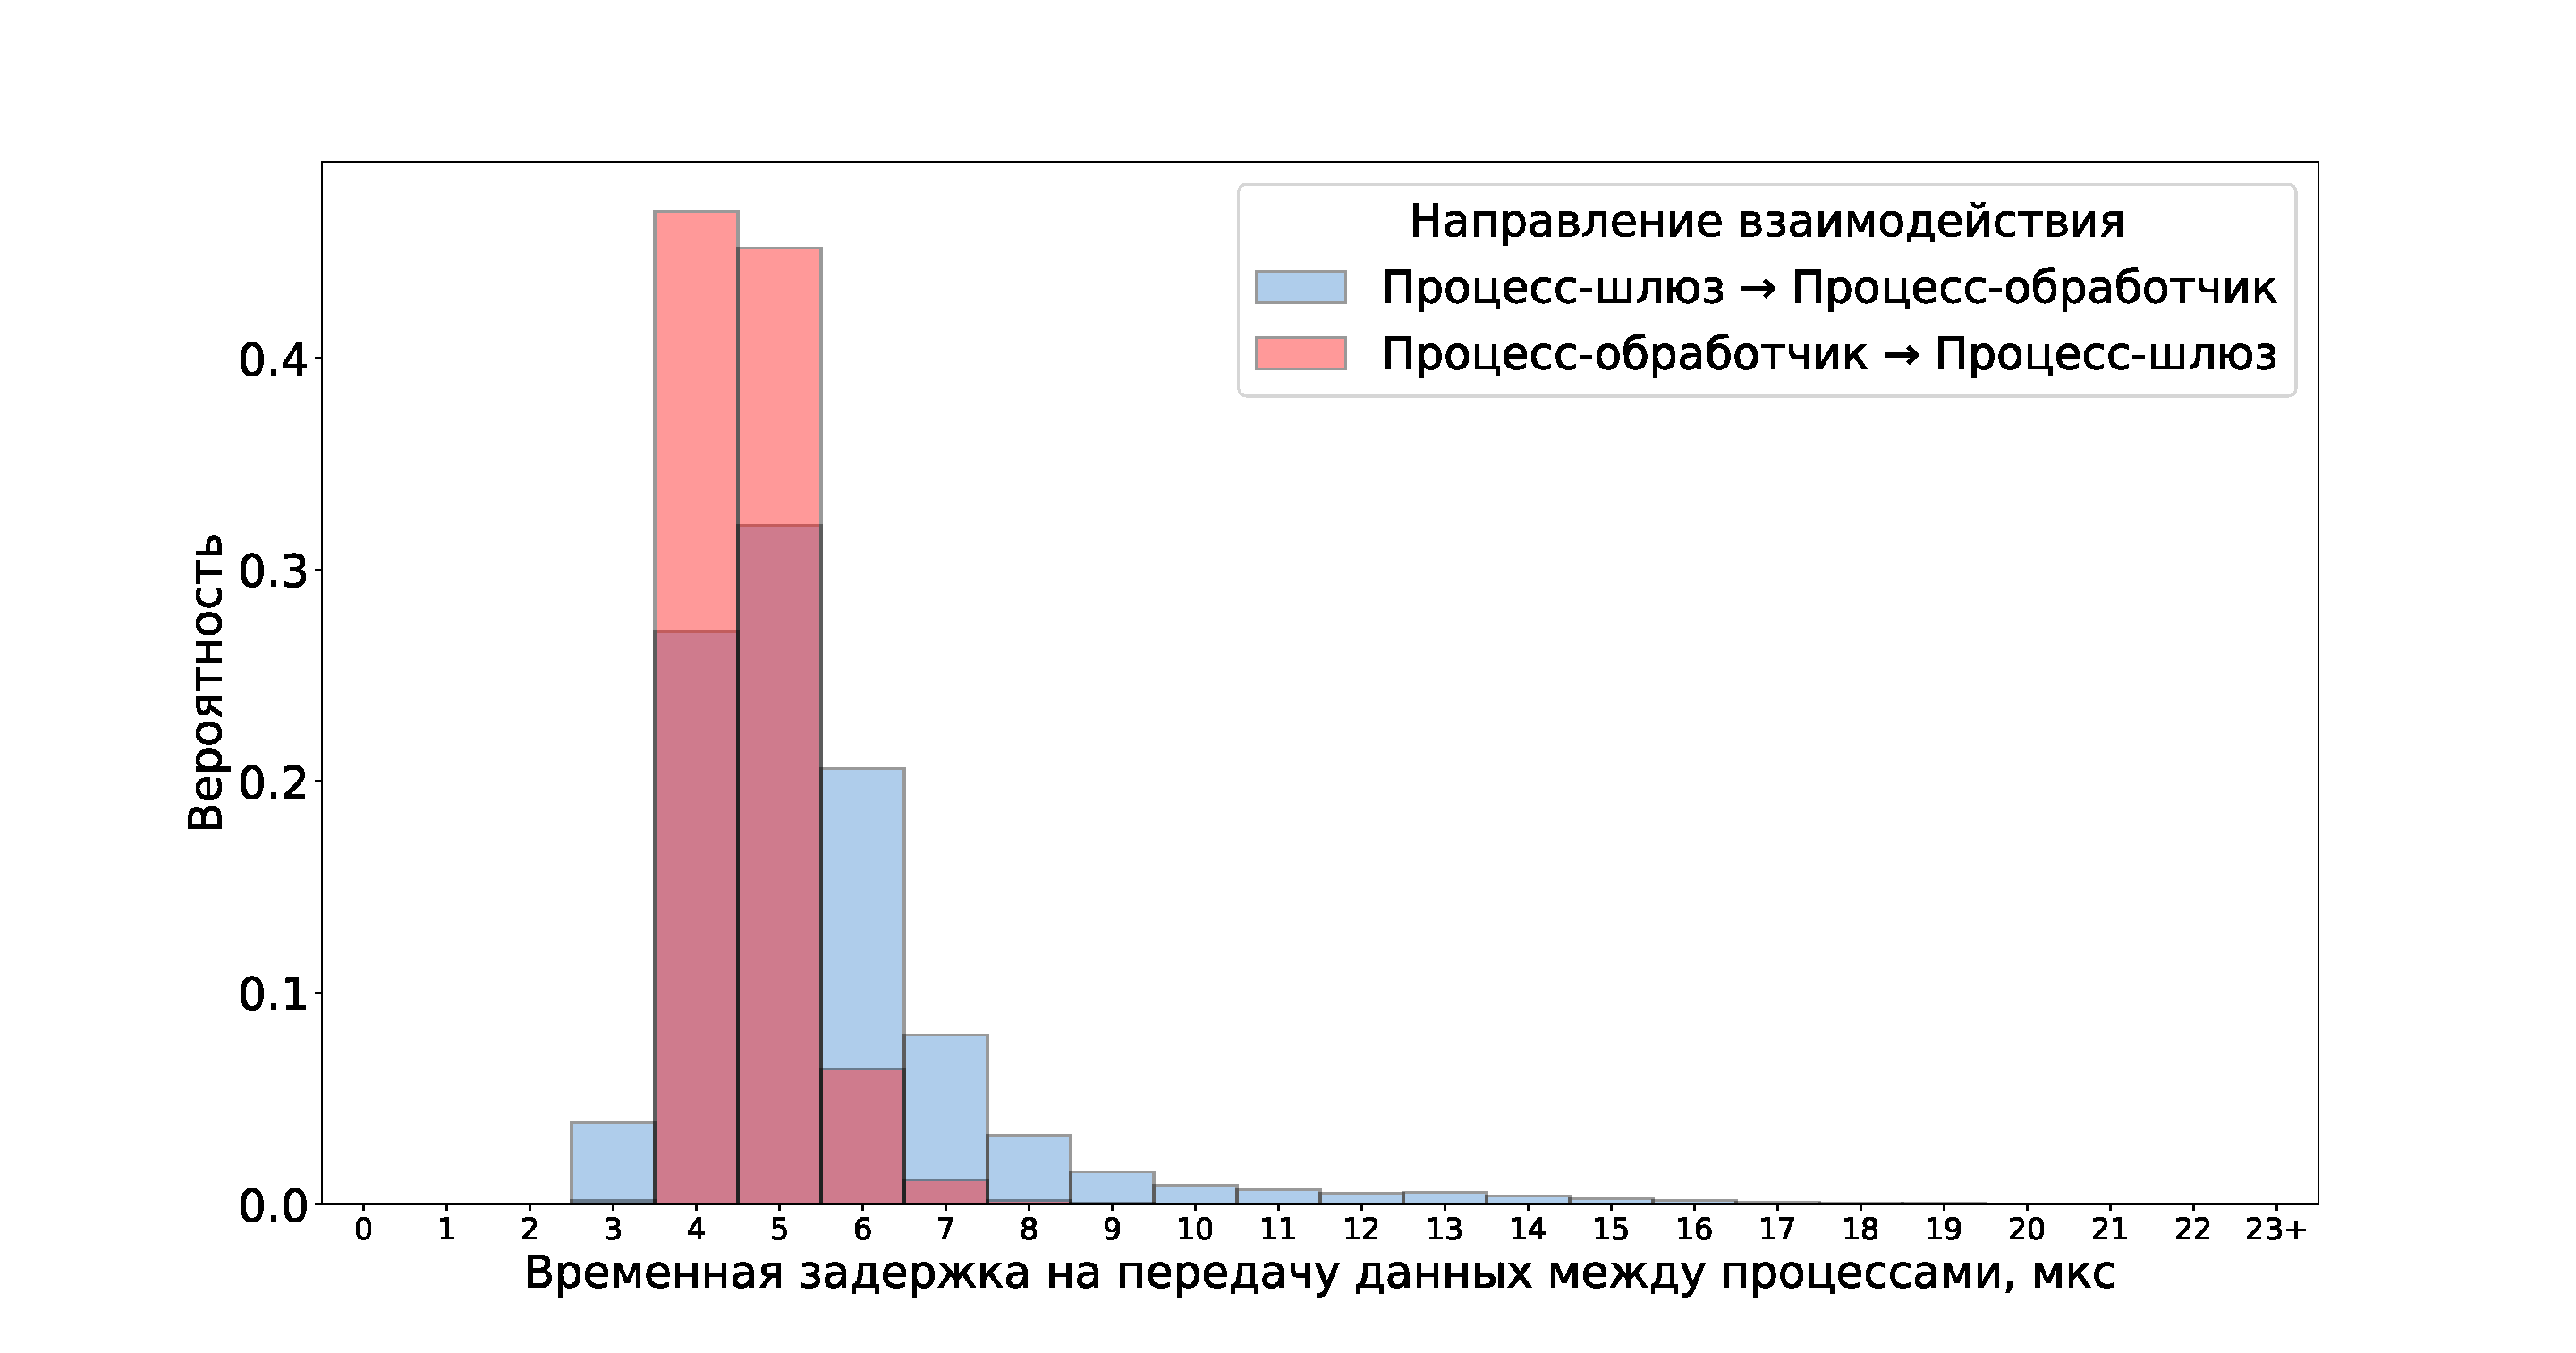
\includegraphics[width=\textwidth]{../../graphics/hist/NonBlockingLF}
\end{figure}

\begin{table}[!h]
\caption{Основные показатели временной задержки на передачу данных между процессами для метода, использующего разделяемую память для передачи данных, неблокирующий мультиплексор в разделяемой памяти и модель ''Лидер/Последователи`` при обслуживании заявок}\label{chapter41:TableNonBlockingLF}
\centering
\begin{tabular}{|l|c|c|}
\hline
\begin{tabular}[c]{@{}l@{}}Направление\\ взаимодействия/\\ Показатель\end{tabular} & \multicolumn{1}{l|}{\begin{tabular}[c]{@{}l@{}}Процесс-шлюз $\rightarrow$\\ Процесс-обработчик\end{tabular}} & \multicolumn{1}{l|}{\begin{tabular}[c]{@{}l@{}}Процесс-обработчик $\rightarrow$\\ Процесс-шлюз\end{tabular}} \\ \hline
min(t), мкс & 1 & 3 \\ \hline
M(t) $\pm$ 95\%, мкс & 6 $\pm$ 2 & 5 $\pm$ 1 \\ \hline
max(t), мс & 0.064 & 0.017 \\ \hline
\begin{tabular}[c]{@{}l@{}}$\Delta$, мс\end{tabular} & 7.1 $\pm$ 5.8 & 7.1 $\pm$ 5.8 \\ \hline
\begin{tabular}[c]{@{}l@{}}$\delta$, мкс\end{tabular} & 220 $\pm$ 197 & 326 $\pm$ 272 \\ \hline
\end{tabular}
\end{table}

Метод с активным ожиданием событий на мультиплексоре в разделяемой памяти ожидаемо показывает лучший результат по сравнению со всеми ранее рассмотренными методами. Это происходит потому что в данном случае нет необходимости пробуждать и дожидаться пробуждения потока для обслуживания заявки. Исходя из разницы временной задержки на передачу данных в неблокирующем и блокирующим методах, пробуждение потока до постановки его на выполнение занимает около 5-6 мкс.
\textbf{TBD: а надо ли оно мне? Вопрос корректности приведения циклов на AMD к секундам спорный}
В работе другого автора \cite{8526899} была измерена временная задержка на пробуждение потоков, прикрепленных к разным ядрам разных процессоров, посредством системного вызова futex. Измерения проводились на процессоре AMD Opteron 6272 и показали $\mu = 24640.5$ машинных циклов от системного вызова до выполнения первой инструкции пробужденным потоком. Или $\frac{24640.5~\text{машинных~циклов}}{2.1~*~10^9~\text{Гц}} \approx 11 ~\text{мкс}$ при частоте процессора 2.1 ГГц, что похоже на обозначенный выше результат с учетом использования в настоящей работе более современного аппаратного обеспечения.

Для данного метода распределение временной задержки на передачу данных от процесса-обработчика к процессу-шлюзу схоже с предыдущими методами, но этот показатель существенно отличается при передаче от процесса-шлюза к процессу-обработчику. Это может быть вызвано тем, что более быстрый метод межпроцессного взаимодействия при данной постановке эксперимента приводит к отсутствию и, как следствие, время обслуживания заявки в транспортном потоке процесса-обработчика не влияет на временную задержку на передачу данных.

Данный подход обладает существенным \textbf{недостатком}. Поскольку поток, активно опрашивающий мультиплексор, исполняется до получения и обработки события, то существует возможность, что планировщик ОС вытеснит этот поток с процессора. Стандартный квант планирования потоков в Linux -- 100 мс. Если событие не будет получено и обработано за это время, то поток может быть вытеснен с процессора и временная задержка на передачу данных увеличится на сотни миллисекунд. Данный недостаток не проявляется в проведенном эксперименте, поскольку что интервал $\Delta$ между сериями заявок значительно меньше 100 мс.

\textbf{TBD: объяснить разброс в интервалах между заявками.}


\chapterconclusion

Проведено экспериментальное сравнение разработанных методов межпроцессного взаимодействия.
\begin{enumerate}
\item Методы межпроцессного взаимодействия, использующие мультиплексор в разделяемой памяти для оповещения о появлении данных в очереди в разделяемой памяти имеют существенно меньшую временную задержку на передачу данных, чем метод, использующий для этого TCP. А именно, $11.5 \pm 6.5 \text{ мкс и } 9.5 \pm 1.5 \text{ мкс}$ для пассивного варианта ''Лидер/Последователи`` против $22.5 \pm 12.5 \text{ мкс и } 27.5 \pm 5.5 \text{ мкс}$ для TCP с передачей данных через очередь в разделяемой памяти.
\item В семействе пассивных методов межпроцессного взаимодействия на основе мультиплексора в разделяемой памяти наименьшую временную задержку на передачу данных показала вариация с использованием метода обслуживания заявок ''Лидер/Последователи``, а именно $11.5 \pm 6.5 \text{ мкс и } 9.5 \pm 1.5 \text{ мкс}$ против $12.5 \pm 5.5 \text{ мкс и } 11.5 \pm 2.5 \text{ мкс}$.
\item Самой низкой временной задержки на передачу данных удалось добиться при использовании активно опрашивающей мультиплексор вариации метода межпроцессного взаимодействия, использующего метод ''Лидер/Последователи`` при обслуживании заявок. А именно, $6 \pm 2 \text{ мкс и } 5 \pm 1 \text{ мкс}$.
\item При использовании пассивных методов на основе мультиплексора в разделяемой памяти заметны эффекты от обслуживания заявок в транспортном потоке на временную задержку на передачу данных. В проведенном эксперименте в процессе-шлюзе заявки частично обслуживаются именно в транспортном потоке, из-за чего могут образовываться очереди и увеличиваться временная задержка на передачу данных. В активно опрашивающем методе этот эффект не заметен, так как временная задержка на передачу данных меньше, соответственно, меньше временная задержка реакции на очередную заявку и, следовательно, меньше возможностей для формирования очереди из заявок.
\item Активно опрашивающий мультиплексор метод обладает существенным недостатком. поток, активно опрашивающий мультиплексор в разделяемой памяти, может быть вытеснен с процессора по окончании отведенного ему кванта процессорного времени -- 100 миллисекунд. В проведенном эксперименте данный эффект не наблюдается, так как серии заявок отправляются симулятором в систему на порядок чаще, каждые $10 \pm 4 \text{ миллисекунд}$. Данный недостаток может быть необходимо разрешить для обеспечения должного уровня качества обслуживания заявок в системе.
\end{enumerate}